%Introduction:

%Briefly explain what an accelerator is and its importance in scientific research
The Proton Synchrotron (PS) is part of the injector chain and used to accelerate particles from the Proton Sychrotron Booster (PSB) to the SPS and finally to the Large Hadron Collider (LHC). For the purpose of CHIMERA, it can also be receive and accelerate heavy ions from the Low Energy Ion Ring (LEIR) and extract them to the East Area. The PS uses radio frequency (RF) cavities to accelerate charged particles, such as protons or Pb ions, to high energies and uses 100 dipoles to bend the beam around it's 628 m circumference \cite{}. These particles are then extracted using slow extraction through a beam line and transported to the CHARM facility where the CHIMERA instruments are located.

%Introduce the concept of beam energy and its significance in the operation of an accelerator
Beam energy refers to the kinetic energy per nucleon $E_{kin}$ of the charged particles beam. The relationship for an ion beam is  $E_{kin, TOT}=E_{kin}\cdot A$, where A is the atomic mass number (A=Z+N, number of protons Z and neutrons N). The total momentum for an ion beam is

$$pc={E_{0}\sqrt{\gamma^{2}-1}}$$

$$pc = E_{0}\sqrt{\left [ \left( \frac{E_{kin}}{E_{0}}+1\right )^{2}-1\right ]}$$

where, $E_{0}$ is the rest mass of the ion and $\gamma=\frac{E}{E_{0}}=\frac{E_{0}+E_{cin}}{E_{0}} = \frac{E_{cin}}{E_{0}}+1$

The rigidity is defined as:
$$B\rho = \frac{pc}{q}$$

\subsubsection{CHIMERA beam}

The CHIMERA beam uses a lead ion beam. It is partially stripped during acceleration Pb54+ (which means it has 54 charges and 28 $e^{-}$ remaining) of isotope A=208 of energy 1 GeV per nucleon the momentum would be:

$$pc = E_{0}\sqrt{\left [ \left( \frac{1\text{ [GeV]}\cdot 208}{E_{0}}+1\right )^{2}-1\right ]}$$

where the rest mass $E_{0}$ of Pb54+ is:

$$m_{Pb54+}= 82\cdot m_{proton} + 126\cdot m_{neutron} + 28\cdot m_{e^{-}} - m_{defect} = 193.74 \frac{\text{GeV}}{\text{c}^{2}}$$

with the mass defect: $m_{defect}=82\cdot m_{proton} + 126\cdot m_{neutron} + 28\cdot m_{e^{-}} - 208\cdot m_{u}$ 

$$m_{p} = 0.93828 \text{ } GeV/c^{2}$$
$$m_{n} = 0.93957 \text{ } GeV/c^{2}$$
$$m_{e^{-}} = 0.000511 \text{ } GeV/c^{2}$$
$$m_{u} = 0.9315 \text{ } GeV/c^{2}$$
\cite{boston_university_nuclear_nodate}

\subsection{Example calculation}

$$B\rho \text{ [T m]} = 3.3356\cdot p \text{ [GeV/c]}$$
where for the PS, $\rho = 70.0789$ m.

Figure \ref{fig:bfield} shows the shape of the magnetic field in the main dipoles of the PS produced by POPS. There is the injection plateau, the flat-top and a spike at the end to circumvent some limitation of POPS.

\begin{figure}[h]
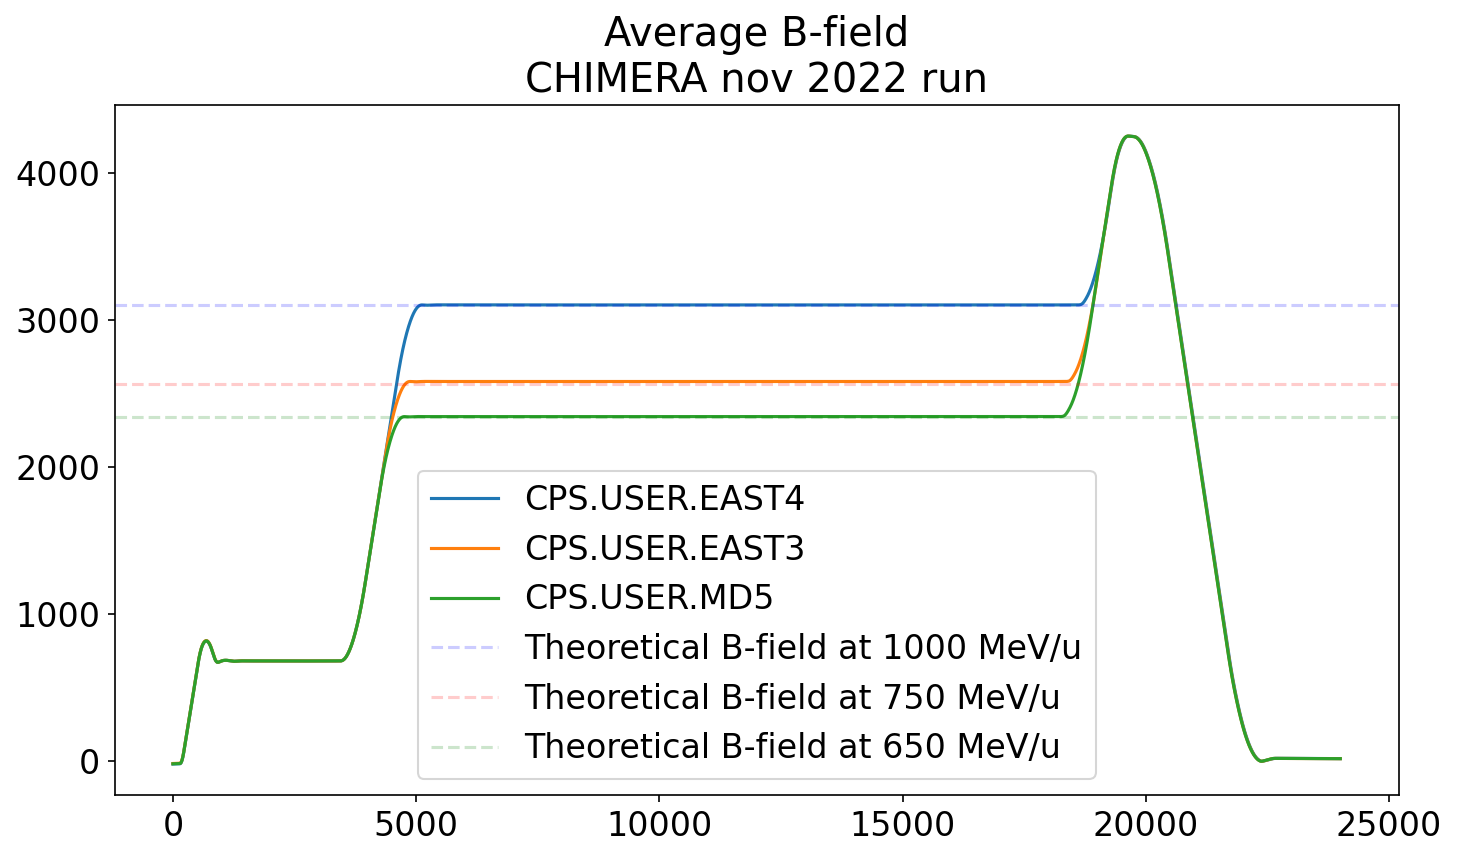
\includegraphics[width=0.9\textwidth]{images/average_b_field_chimera.png}
\caption{CHIMERA B-field for different energies}
\label{fig:bfield}
\end{figure}

\subsubsection{Energy scan}

For development purposes and after the ESA run, we ramped the beam energy using an automatic script.

\begin{figure}[h]
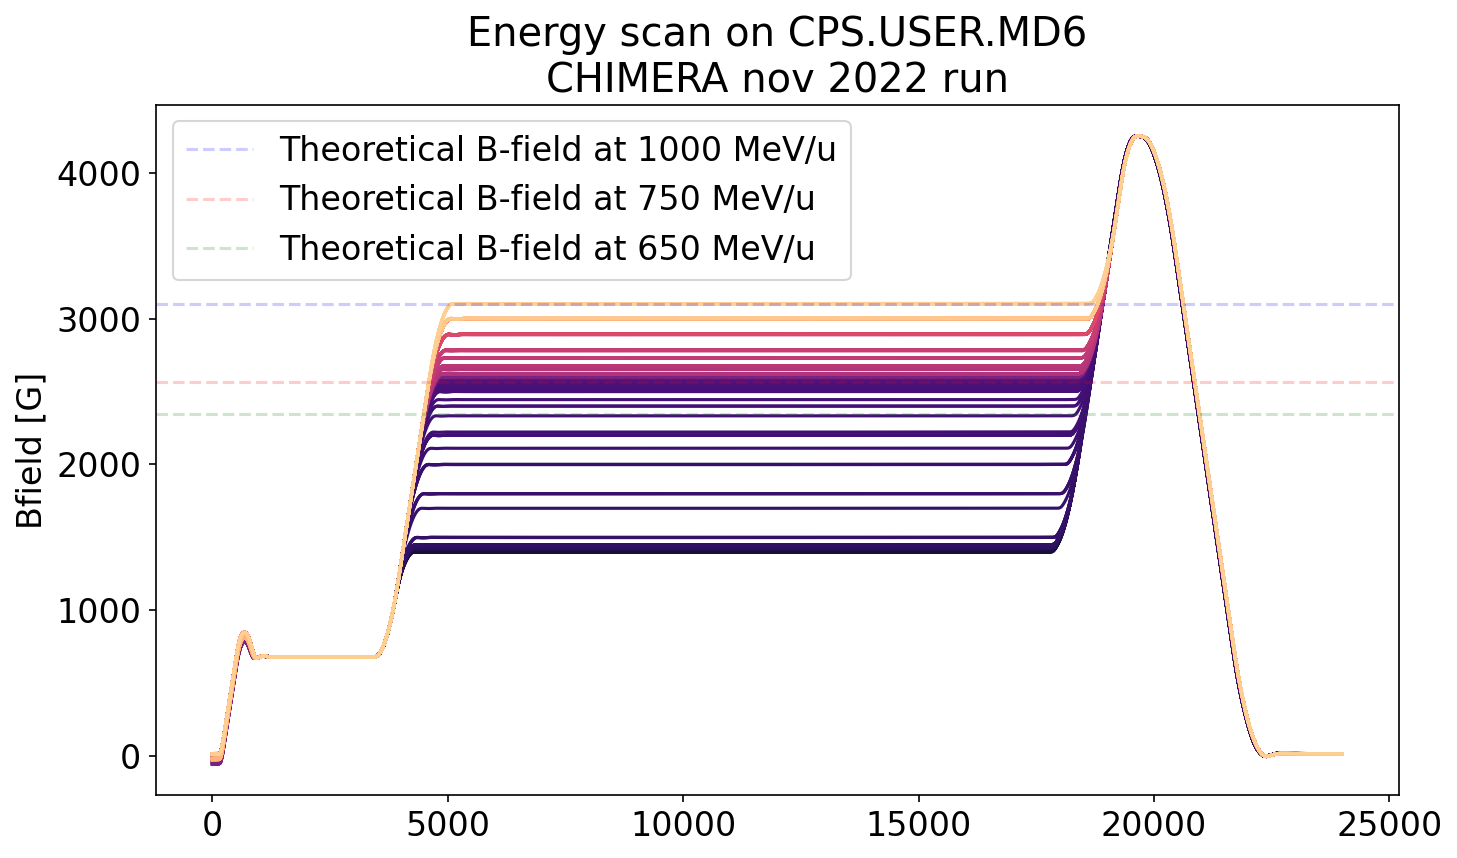
\includegraphics[width=0.9\textwidth]{images/energy_scan_chimera 1.png}
\caption{CHIMERA B-field for different energies}
\label{fig:bfield}
\end{figure}


\begin{figure}[h]
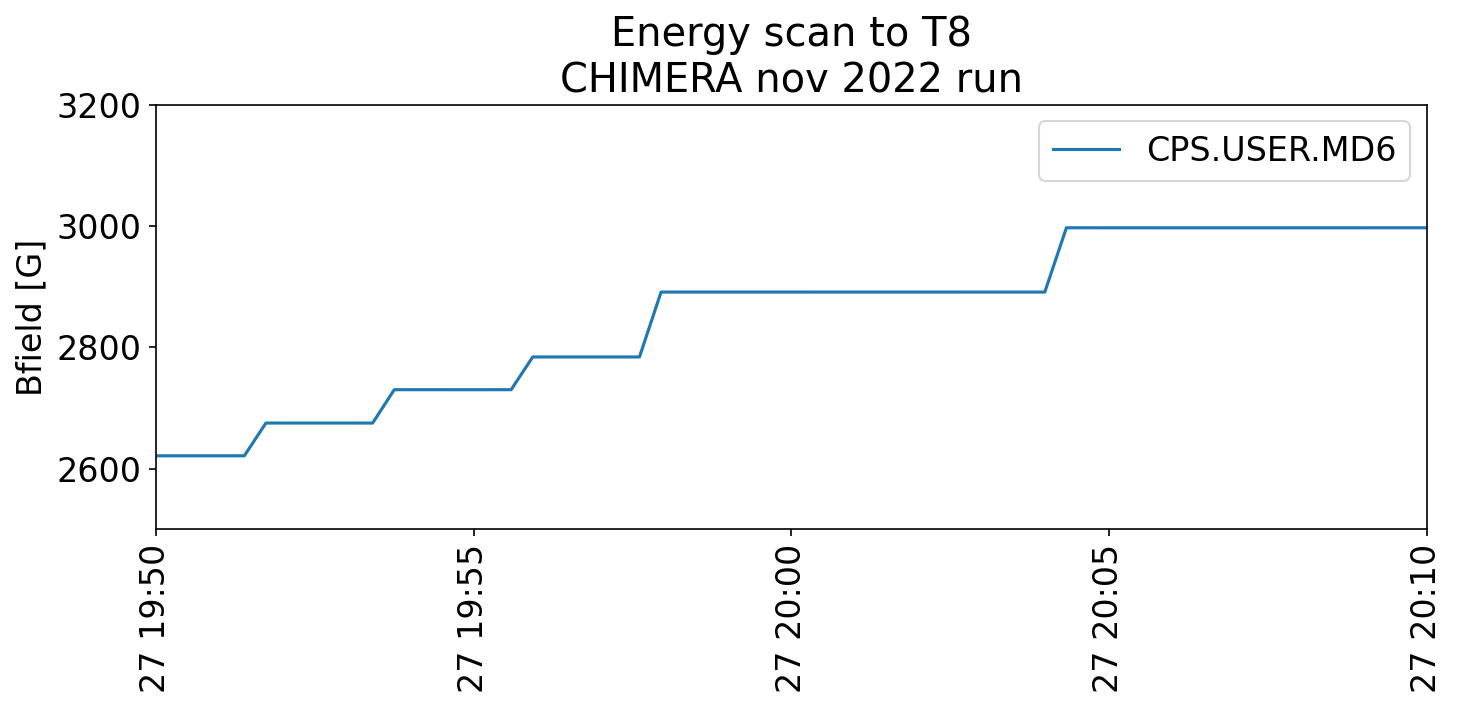
\includegraphics[width=0.9\textwidth]{images/energy_scan_timestamp_chimera 1.png}
\caption{CHIMERA B-field for different energies}
\label{fig:bfield}
\end{figure}
